\section{The Two Coordinates}
\label{sec:coordinates}

\subsection{Notation}
Players $i\in\{1,\dots,N\}$ with finite action sets $A_i$, $|A_i|=m_i$; mixed strategies
$\sigma_i\in\Delta(A_i)$ with full support. Expected payoffs
$U_i(a;\sigma_{-i})=\sum_{a_{-i}}\big(\prod_{j\ne i}\sigma_j(a_j)\big)u_i(a,a_{-i})$, and
logit QRE
\begin{equation}
\sigma_i(a)=\frac{\exp\{\lambda_i U_i(a;\sigma_{-i})\}}{\sum_{b}\exp\{\lambda_i U_i(b;\sigma_{-i})\}}.
\label{eq:qre}
\end{equation}
Write $C_i:=\operatorname{diag}(\sigma_i)-\sigma_i\sigma_i^{\top}$ for the choice
covariance, $S:=\operatorname{blockdiag}(\lambda_i C_i)$, and
$B_{ij}(a,b):=\partial U_i(a;\sigma_{-i})/\partial\sigma_j(b)$ for $j\ne i$, $B_{ii}:=0$.
$C_i$ is rank-deficient by construction, so all linear algebra below is performed on the
tangent space $T=\bigoplus_i\{v:\mathbf{1}^{\top}v=0\}$ in an explicit Helmert basis;
omitting that projection fabricates a zero eigenvalue and a spurious criticality reading.

\subsection{The local coordinate}
The exact static identity $\chipart_i=\partial\sigma_i/\partial h_i|_{\sigma_{-i}}=\lambda_i C_i$
is a fluctuation--dissipation relation with opponents frozen. Total differentiation of
Equation~\eqref{eq:qre} under a payoff field $h$ gives $d\sigma=S(dh+B\,d\sigma)$, hence the
\emph{strategic resolvent}
\begin{equation}
\chieq:=\frac{d\sigma^*}{dh}=(I-SB)^{-1}S .
\label{eq:resolvent}
\end{equation}
$\chieq$ is symmetric if and only if $S(B-B^{\top})S=0$, which under full support and on $T$
is equivalent to $B=B^{\top}$, i.e.\ to the normalised game having zero harmonic component.
Strategic feedback therefore neither creates nor destroys reciprocity, and the departure is
observable. Define the \emph{response asymmetry}
\begin{equation}
\R:=\frac{\|\chieq-(\chieq)^{\top}\|_F}{\|\chieq+(\chieq)^{\top}\|_F}.
\label{eq:R}
\end{equation}
$\R$ is estimable from cross-agent pass-through asymmetry---how much agent $i$ moves when
agent $j$'s cost moves, against the reverse---without knowing payoffs. Its \emph{zero test}
is $\lambda$-free; its magnitude is not, and reporting a magnitude without the $\lambda$ it
was read at is an error.

\subsection{The global coordinate}
Logit revision defines a Glauber jump process on the joint profile space with
$N_{\mathrm{states}}=\prod_i m_i$. At stationarity the pairwise current is
$J^*(a,a')=\pi^*(a)w(a\!\to\!a')-\pi^*(a')w(a'\!\to\!a)$ and the entropy production rate is
\begin{equation}
\EPR=\tfrac12\sum_{a,a'}\big[\pi^*(a)w(a\!\to\!a')-\pi^*(a')w(a'\!\to\!a)\big]
\log\frac{\pi^*(a)w(a\!\to\!a')}{\pi^*(a')w(a'\!\to\!a)}\;\ge\;0 ,
\label{eq:epr}
\end{equation}
non-negative by construction and zero exactly under detailed balance. From observed
trajectories alone we use a $k$-block KLD estimator and a debiased finite-time
thermodynamic-uncertainty lower bound~\cite{barato2015}; the latter is a certified bound
rather than a point estimate and degrades gracefully under partial observation.

\subsection{The confound, and why it must be conditioned away}
Both coordinates are monotone in the harmonic fraction
$\alpha(u):=\|u^H\|/(\|u^P\|+\|u^H\|)$ of the normalised game's Candogan
decomposition~\cite{candogan2011}, computed here by a separable Kronecker transform in
near-linear time. Any unconditional correlation between $\R$ and $\EPR$ is therefore
substantially a correlation of each with $\alpha$. \textbf{The entire empirical design of
this paper is the decision to stratify on $\alpha$ before comparing them.}

\subsection{The plane}
Equations~\eqref{eq:R} and~\eqref{eq:epr} define a map from a game (or an observed system)
to a point in the quadrant $[0,\infty)^2$. Figure~\ref{fig:routes} shows the two
computational routes; they share an origin and are otherwise unrelated in type---one is a
derivative evaluated at a single equilibrium, the other a functional of a flux field over
the whole profile space.

\begin{figure}[H]
\centering
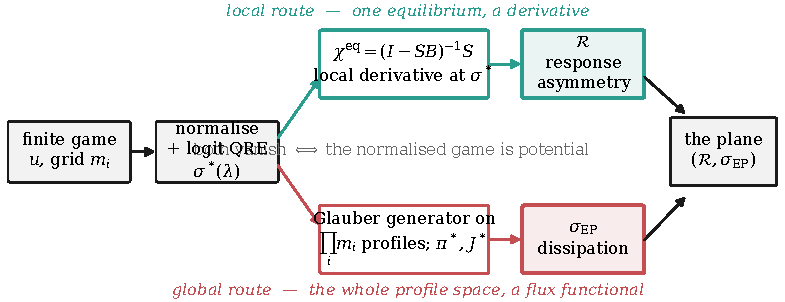
\includegraphics[width=\linewidth]{figures/fig1_two_routes.pdf}
\caption{The two routes from a finite game to a coordinate. Both terminate in zero exactly
when the normalised game is potential; nothing else forces them to agree.}
\label{fig:routes}
\end{figure}
